% Provenance (never printed): see sources/outline_sources.md (Year 2: the long-term carbon cycle
% and the silicate-weathering thermostat; Palaeozoic glaciations; the Cretaceous greenhouse; the
% PETM; Cenozoic cooling). Reservoirs from IPCC AR6 WG1 Figure 5.12; long-term fluxes after Derry
% (2024); weathering laws after Colbourn and others (2013); Phanerozoic CO2 after Foster and
% others (2017); Phanerozoic temperatures after Judd and others (2024); Cenozoic isotopes from
% CENOGRID (Westerhold 2020); the Eocene--Oligocene transition after Hutchinson and others (2021);
% the PETM after AR6 WG1 chapters 2 and 5. The thermostat model, its curves and every number of
% the exercises and problem from figdata/bachelor-2/deeptime.py and the Book 4 second-writer
% scratch calculator calc/ch26.py.
\chapter{المناخ عبر الزمن الجيولوجي}\label{ch:b2:deep-time-climate}

قبل خمسين مليون سنة لم يكن أيّ غطاء جليدي قائمًا في أيّ مكان على الأرض. وكان الهواء يحتوي على أكثر من
ألف جزء في المليون من ثنائي أكسيد الكربون، وكان القطبان قد احترّا أكثر بكثير من خطّ الاستواء،
وكانت غابات من نوع شبه مداري تنمو عند \ang{70}~جنوبًا، طوال أشهر الليل القطبي. وقبل أربعة وثلاثين
مليون سنة امتدّ الجليد فوق القارّة القطبية الجنوبية، ولم يغادرها منذئذ. وعلى مدى مئات الملايين
من السنين المسجّلة في الصخور، تأرجحت الأرض بين عوالم كهذه، بجليد ومن دون جليد؛ ومع ذلك
لم تُغلِ محيطاتها حتى تتبخّر قطّ، ولم تتجمّد نهائيًا منذ كرات الثلج في
\cref{ch:b2:precambrian-earth}. يتتبّع هذا الفصل الكربون الذي يحدّد هذه المناخات، والدورة البطيئة
التي تنقله بين الهواء والصخور، ومنظّم الحرارة الذي يُبقي الكوكب
صالحًا للحياة.
% ledger: ipcc:ref-periods, ar6ch2:cenozoic, hutchinson21:eot

\begin{recall}
\textbf{من مجلّدات المدرسة}: أثر الدفيئة والتأثير الإشعاعي؛ وتأثير
ثنائي أكسيد الكربون يزداد مع لوغاريتم تركيزه، \qty{3.93}{W.m^{-2}} لكلّ مضاعفة؛
وحساسية المناخ عند التوازن، وأفضل تقدير لها \qty{3}{\celsius}؛ وانطلاق الغازات؛ والدورات الجليدية
والذروة الجليدية الأخيرة. \textbf{من مجلد السنة الأولى}: التجوية الكيميائية
والتحلّل المائي للسيليكات؛ والمعادن الطينية؛ والرسوبات الكلسية الناعمة، والحدّ الانحلالي وعمق
التعويض الكربوناتي. \textbf{من الفصول السابقة}: الشمس الفتية الخافتة \omterm{def:b2:precambrian-earth:snowball}{والأرض الكرة الثلجية}
(\cref{ch:b2:precambrian-earth})؛ \omterm{def:b2:phanerozoic-earth:palaeogeography}{والجغرافيا القديمة} \omterm{def:b2:phanerozoic-earth:oae}{وأحداث نقص الأكسجين المحيطي}
(\cref{ch:b2:phanerozoic-earth})؛ والمؤشّرات المناخية البديلة، و\mbox{\textdir TLT $\delta^{18}$O} \omterm{def:b2:climate-proxies:ice-volume}{وأثر حجم الجليد}
(\cref{ch:b2:climate-proxies})؛ والتأثير المداري (\cref{ch:b2:orbital-forcing}). أمّا دورة الكربون،
وخزّاناتها وزمن المكوث فتنتمي إلى كتب الأحياء، وقانون أرينيوس إلى
كتب الكيمياء.
\end{recall}
% ledger: ipcc:erf-2xco2, ipcc:log-co2, ipcc:ecs

\section{الدورة الطويلة الأمد للكربون}\label{sec:b2:deep-time-climate:cycle}

\subsection*{الخزّانات والتدفّقات}

\begin{definition}[الدورة الطويلة الأمد للكربون؛ دورة الكربونات والسيليكات]\label{def:b2:deep-time-climate:carbon-cycle}
\emph{الدورة الطويلة الأمد للكربون}\index{الدورة الطويلة الأمد للكربون} هي تبادل الكربون بين
الخزّانات السطحية (الغلاف الجوي والمحيط والغلاف الحيوي والتربة) والأرض الصلبة: انطلاق الغازات البركاني
والتحوّلي، وتجوية الصخور، ودفن الكربون الكربوناتي والعضوي في
رواسب تصير لاحقًا صخورًا أو تندسّ. وتدفّقاتها صغيرة إزاء الخزّانات
السطحية وتعمل على مدى $10^5$ إلى $10^8$ سنة. و\emph{دورة الكربونات
والسيليكات}\index{دورة الكربونات والسيليكات} هي جزؤها غير العضوي: يغادر ثنائي أكسيد الكربون الوشاح
والقشرة عند البراكين، وتستهلكه تجوية صخور السيليكات، ويترسّب على
قاع البحر كربوناتٍ، ويعود إلى السطح حين تتحوّل تلك الكربونات أو
تندسّ فتنطلق غازاتها.
\end{definition}
% ledger: derry24:fluxes, derry24:subduction, colbourn13:timescale

تتتبّع كتب الأحياء الكربون عبر التمثيل الضوئي والتنفّس والمحيط على مدى سنوات إلى
قرون. وعلى المقياس الزمني لتاريخ المناخ تتّسع الصورة لتشمل الصخور. فقبل
العصر الصناعي كان الغلاف الجوي يحتوي على \qty{591}{PgC} (بيتاغرامات، أي مليارات الأطنان، من الكربون)؛
وكان المحيط يحتوي على \num{38700}، كلّها تقريبًا كربونًا غير عضوي مذابًا في المياه المتوسطة
والعميقة (\num{37100})؛ وكانت النباتات والتربة والتربة الصقيعية تحتوي معًا على \num{3350}.
والخزّانات السطحية النشطة معًا تحتوي على نحو \num{3.5e6} تيرامول من الكربون، أي نحو
\qty{42000}{PgC}. والصخور الرسوبية تحتوي على الكربون أيضًا، على هيئة حجر جيري وعلى هيئة مادة عضوية
مبعثرة في الطفل الصفحي، ولا تتبادله مع السطح إلا ببطء.
% ledger: ar6ch5:fig512, derry24:residence

يجري تقدير حديث للمدخلات والمخرجات، بالتيرامول من الكربون في السنة ($\qty{1}{Tmol}$ من
الكربون يساوي \qty{0.012}{PgC})، على النحو الآتي. إلى المحيط والغلاف الجوي: انطلاق الغازات البركاني عند
الظهرات وسط المحيطية (1.3)، والجزر المحيطية (1.3)، والأقواس (4.5) والوديان الخسفية القارية (4.2)، أي نحو 11
إجمالًا؛ وانطلاق الغازات التحوّلي، من 2 إلى 4؛ وتجوية الكربونات القديمة، 12.3، وأكسدة
الكربون العضوي القديم الذي يكشفه الحتّ، 8.1، مع 2.0 من الميثان الجيولوجي: \num{36.7} إجمالًا.
وخروجًا منهما: ترسّب الكربونات، نحو 26، ودفن الكربون العضوي، نحو 16. والجانبان
متوازنان ضمن حدود الشكّ فيهما. ولا يقدّم انطلاق الغازات من باطن الأرض إلا ما يزيد قليلًا على
ثلث المدخلات (\cref{exo:b2:deep-time-climate:2})؛ والباقي كربون رسوبي قديم في
دورته من جديد. وتقديرات أخرى للتدفّق البركاني أدنى، \qty{0.1}{PgC} في السنة
(نحو 8 تيرامول) في الميزانية العالمية للكربون لدى الهيئة الحكومية الدولية المعنية بتغيّر المناخ، أو \qty{0.26}{Gt} من ثنائي أكسيد الكربون (نحو 6
تيرامول من الكربون) في مسح لهيئة المسح الجيولوجي الأمريكية: فالمدخل البركاني معروف ضمن
عامل اثنين.
% ledger: derry24:fluxes, ar6ch5:fig512, usgs:volcanic-co2

\begin{omfigure}
\centering
\begin{tikzpicture}[font=\scriptsize, >={Stealth[length=2mm]},
  box/.style={draw, thick, rounded corners=2pt, align=center, inner sep=4pt},
  up/.style={->, very thick, omThm}, down/.style={<-, very thick, omDef},
  lab/.style={midway, above, sloped, font=\scriptsize}]
% reservoirs: ar6ch5:fig512; active reservoirs derry24:residence; fluxes derry24:fluxes, derry24:subduction
\draw[thick, rounded corners=2pt, fill=blue!6] (-6.3,0) rectangle (6.0,2.6);
\node[anchor=north west, font=\small\bfseries] at (-6.2,2.55) {\foreignlanguage{arabic}{الخزّانات السطحية، نحو \qty{42000}{PgC}}};
\node[box, fill=white] (atm) at (-4.6,1.45) {الغلاف الجوي\\\qty{591}{PgC}};
\node[box, fill=white] (oc) at (0.6,1.45) {المحيط\\\qty{38700}{PgC}};
\node[box, fill=white] (land) at (4.3,1.45) {\foreignlanguage{arabic}{النباتات، والتربة،}\\\foreignlanguage{arabic}{والتربة الصقيعية \qty{3350}{PgC}}};
\draw[->, very thick, omProp] (atm.east) -- (oc.west);
\node[align=center, text=omProp] at (-2.0,0.6) {\foreignlanguage{arabic}{تجوية السيليكات 11--12، على هيئة بيكربونات}};
\draw[<->, thick, black!50] (oc.east) -- (land.west);
% sedimentary rocks and mantle
\node[box, fill=brown!12, minimum width=5.7cm, minimum height=1.1cm] (rock) at (-3.35,-4.55) {\foreignlanguage{arabic}{الصخور الرسوبية:}\\كربونات وكربون عضوي};
\node[box, fill=orange!15, minimum width=3.0cm, minimum height=1.1cm] (mantle) at (4.3,-4.55) {الوشاح};
% inputs (red, up) and outputs (blue, drawn upwards with the tip at the start)
\draw[up] (-5.7,-4.0) -- node[lab] {\foreignlanguage{arabic}{تجوية الكربونات 12.3}} (-5.7,0);
\draw[up] (-4.8,-4.0) -- node[lab] {\foreignlanguage{arabic}{أكسدة كربون عضوي قديم 8.1}} (-4.8,0);
\draw[up] (-3.9,-4.0) -- node[lab] {\foreignlanguage{arabic}{الميثان الجيولوجي 2.0}} (-3.9,0);
\draw[up] (-3.0,-4.0) -- node[lab] {\foreignlanguage{arabic}{انطلاق الغازات التحوّلي 2--4}} (-3.0,0);
\draw[down] (-1.9,-4.0) -- node[lab] {\foreignlanguage{arabic}{ترسّب الكربونات 26}} (-1.9,0);
\draw[down] (-1.0,-4.0) -- node[lab] {\foreignlanguage{arabic}{دفن الكربون العضوي 16}} (-1.0,0);
\draw[up] (4.3,-4.0) -- node[lab] {\foreignlanguage{arabic}{البراكين والوديان الخسفية 11.3}} (4.3,0);
\draw[->, very thick, black!70] (rock.east) -- node[above] {\foreignlanguage{arabic}{الاندساس 4--6}} (mantle.west);
\end{tikzpicture}
\par\smallskip{\small \omterm{def:b2:deep-time-climate:carbon-cycle}{الدورة الطويلة الأمد للكربون}، مع خزّانات ما قبل الصناعة من الميزانية
العالمية للكربون لدى الهيئة الحكومية الدولية المعنية بتغيّر المناخ، والتدفّقات الحالية من توليفة عام 2024، بالتيرامول من الكربون في السنة
(\qty{1}{Tmol.yr^{-1}} = \qty{0.012}{PgC.yr^{-1}}). الأحمر: المدخلات إلى الخزّانات السطحية؛ والأزرق:
المخرجات. وتجوية السيليكات لا تغادر السطح: فهي تنقل الكربون من الهواء إلى
المحيط على هيئة بيكربونات، ثم يغادره على هيئة رسوبيات كربوناتية.}
\end{omfigure}

إذا قُسمت الكمّية \qty{3.5e6}{Tmol} في الخزّانات السطحية على التدفّق المارّ بها، أعطت
زمن مكوث للكربون من 8 إلى \num{9e4} سنة. فالكربون الذي يدخل المحيط والهواء يُدفن
من جديد في غضون نحو مئة ألف سنة، وهي طرفة عين على مقياس هذا الفصل: فالخزّانات
السطحية تتبع المدخلات والمخرجات البطيئة عن كثب، وأيّ اختلال دائم بينها
يغيّر ثنائي أكسيد الكربون في الهواء.
% ledger: derry24:residence

\subsection*{تجوية الكربونات وتجوية السيليكات}

يذيب المطر ثنائي أكسيد الكربون ويهاجم الصخور، كما وصف مجلد السنة الأولى. ونوعان من الصخور
يسلكان سلوكين مختلفين جدًّا. فتجوية حجر جيري تأخذ ثنائي أكسيد كربون واحدًا من الهواء وكربونًا
واحدًا من الصخر إلى الماء؛ وحين يبني كائن بحري صدفته من النواتج،
يعود كربون واحد إلى الهواء:
\[
  \ce{CaCO3 + CO2 + H2O -> Ca^{2+} + 2 HCO3^-} , \qquad
  \ce{Ca^{2+} + 2 HCO3^- -> CaCO3 + CO2 + H2O} .
\]
فالرحلة ذهابًا وإيابًا معدومة الأثر بالنسبة إلى الهواء. أمّا تجوية سيليكات، مكتوبة هنا بالولاستونيت
بديلًا من سيليكات الكالسيوم في الغرانيت والبازلت، فتأخذ هي أيضًا ثنائي أكسيد الكربون، لكنها لا تأتي
بشيء منه من الصخر:
\[
  \ce{CaSiO3 + 2 CO2 + H2O -> Ca^{2+} + 2 HCO3^- + SiO2} ,
\]
والكربونات المبنيّة منها لا تعيد إلا واحدًا من الاثنين:
\[
  \ce{CaSiO3 + CO2 -> CaCO3 + SiO2} \quad\text{(صافٍ)} .
\]
فكلّ مول من سيليكات الكالسيوم أو المغنيسيوم يتعرّض للتجوية على اليابسة يحبس إذن مولًا واحدًا من ثنائي أكسيد الكربون
في صخر كربوناتي. ولهذا يزيد ترسّب الكربونات، نحو 26، على تجوية الكربونات،
12.3، بما يقارب 11 إلى 12 تيرامولًا في السنة تستهلكها تجوية السيليكات؛ وتجوية
السيليكات، لا الكربونات، هي التي توازن البراكين على مدى ملايين السنين.
% ledger: colbourn13:timescale, derry24:fluxes

\section{منظّم الحرارة بتجوية السيليكات}\label{sec:b2:deep-time-climate:thermostat}

\subsection*{تغذية راجعة سالبة}

تجوية السيليكات تفاعل كيميائي، وهي ككثير من التفاعلات أسرع حين يكون الجوّ دافئًا. والدفء
يجلب أيضًا مزيدًا من المطر والجريان السطحي، اللذين يحملان النواتج بعيدًا ويأتيان بماء عذب إلى
الصخر. فيرتفع المعدّل إذن مع درجة الحرارة؛ ودرجة الحرارة ترتفع مع ثنائي أكسيد الكربون في
الهواء. فكوكب يكتسب ثنائي أكسيد الكربون يحترّ، ويتعرّض للتجوية أسرع، ويفقده من جديد.

\begin{definition}[منظّم الحرارة بتجوية السيليكات]\label{def:b2:deep-time-climate:thermostat}
\emph{منظّم الحرارة بتجوية السيليكات}\index{منظّم الحرارة بتجوية السيليكات} هو التغذية الراجعة
السالبة بين المناخ \omterm{def:b2:deep-time-climate:carbon-cycle}{والدورة الطويلة الأمد للكربون}: فتجوية صخور السيليكات، التي
تنزع ثنائي أكسيد الكربون من الغلاف الجوي إلى صخر كربوناتي، تزداد مع درجة الحرارة
والجريان السطحي، فيرفع ارتفاعُ ثنائي أكسيد الكربون الجوّي معدّلَ نزعه هو نفسه
ويخفضه انخفاضُه. وعلى مدى $10^5$ إلى $10^6$ سنة يعيد النزعَ إلى التوازن مع
انطلاق الغازات.
\end{definition}
% ledger: colbourn13:timescale, colbourn13:weathering, hutchinson21:gateways

الاعتماد على درجة الحرارة هو اعتماد قانون أرينيوس في كتب الكيمياء. فمع طاقة
تنشيط $E_{\text a}$ لانحلال سيليكات الكالسيوم والمغنيسيوم، يكون تدفّق التجوية عند
درجة حرارة $T$ قريبة من درجة مرجعية $T_0$ هو
\[
  W = W_0 \exp\Bigl[-\frac{E_{\text a}}{R}\Bigl(\frac1T - \frac1{T_0}\Bigr)\Bigr]
  \approx W_0\, e^{k_T (T - T_0)}, \qquad k_T = \frac{E_{\text a}}{R T_0^2},
\]
لأن $1/T - 1/T_0 \approx -(T - T_0)/T_0^2$. ويعطي الانحلال في المختبر $E_{\text a} =
\qty{63}{kJ.mol^{-1}}$، ومع $T_0 = \qty{288}{K}$، $k_T = \qty{0.09}{K^{-1}}$: فيزداد التدفّق
بنحو \qty{9}{\percent} لكلّ درجة؛ وضمن عشر درجات من $T_0$ يبتعد التقريب
عن القانون الدقيق بأقلّ من \qty{3}{\percent} (\cref{exo:b2:deep-time-climate:6}). وتقدير ميداني هو
$74 \pm \qty{29}{kJ.mol^{-1}}$، فالحساسية غير مؤكّدة بعامل اثنين تقريبًا. والجريان السطحي
يضيف إليها: مع تدفّق يتناسب مع $(R/R_0)^{0.65}$ وجريان سطحي يرتفع بنسبة
\qty{4.5}{\percent} لكلّ درجة، تصبح الحساسية المجمّعة $k = 0.09 + 0.65\times0.045 =
\qty{0.119}{K^{-1}}$.
% ledger: colbourn13:weathering
% values: k_run 0.11925 (deeptime.py)

\subsection*{نموذج بخزّان واحد}

لنرَ مدى سرعة عمل منظّم الحرارة، نتتبّع الكربون الفائض $M$ الذي يحتويه المحيط والغلاف الجوي
فوق حالة مستقرّة. ففي غضون بضعة آلاف من السنين بعد اضطراب يكون المحيط وكربونات قاع البحر
قد أخرجا معظم الفائض من الهواء؛ ولإطلاق \qty{4000}{PgC}، يبقى نحو
\qty{8}{\percent} في الهواء إلى أن تنزعه تجوية السيليكات. لنكتب $f$ لهذا
الكسر و$A_0 = \qty{591}{PgC}$ لكربون الهواء قبل الصناعة، فيكون ثنائي أكسيد الكربون
في الهواء $C = C_0(1 + fM/A_0)$. ويتبع الاحترار القانون اللوغاريتمي مع حساسية
المناخ $S$، $\Delta T = S\log_2(C/C_0)$، وتتبع التجوية القانون الأسّي أعلاه.
% ledger: colbourn13:timescale, ar6ch5:fig512, ipcc:ecs, ipcc:log-co2

\begin{proposition}[الحالة المستقرّة لمنظّم الحرارة وثابته الزمني]\label{prop:b2:deep-time-climate:thermostat}
ليتغيّر الكربون الفائض $M$ في المحيط والغلاف الجوي وفق
\[
  \frac{\mathrm dM}{\mathrm dt} = V - W_0\,e^{k\,\Delta T(M)}, \qquad
  \Delta T(M) = S\log_2\Bigl(1 + \frac{fM}{A_0}\Bigr),
\]
حيث $V$ انطلاق الغازات و$W_0$ التجوية عند $M = 0$.
\begin{enumerate}
  \item للحالة المستقرّة $\Delta T^* = \ln(V/W_0)/k$، أيًّا كانت $S$ و$f$.
  \item إذا كان $V = W_0$، يضمحلّ فائض صغير وفق $M(t) = M(0)\,e^{-t/\tau}$ مع
        \[
          \tau = \frac{A_0 \ln 2}{f\,k\,S\,W_0} .
        \]
\end{enumerate}
\end{proposition}

\begin{proof}
(1) في حالة مستقرّة $\mathrm dM/\mathrm dt = 0$، فيكون $W_0e^{k\Delta T^*} = V$ و$\Delta T^* =
\ln(V/W_0)/k$؛ ولا تدخل فيه $S$ ولا $f$. (2) قرب $M = 0$، $\log_2(1 + x) \approx x/\ln 2$، فيكون
$\Delta T \approx SfM/(A_0\ln 2)$ و$e^{k\Delta T} \approx 1 + kSfM/(A_0\ln2)$. ومع $V = W_0$
تصبح المعادلة $\mathrm dM/\mathrm dt = -W_0kSfM/(A_0\ln 2) = -M/\tau$، وحلّها هو
الدالة الأسّية.
\end{proof}

النتيجة الأولى هي قلب منظّم الحرارة. فهي تثبّت درجة حرارة، لا تركيزًا: فإذا أطلقت
البراكين غازات أكثر بنسبة \qty{20}{\percent}، استقرّت الأرض أدفأ بمقدار $\ln 1.2/0.09 = \qty{2.0}{\celsius}$،
أيًّا كانت حساسيتها المناخية، ويتكيّف ثنائي أكسيد الكربون مع ما يعطي ذلك
الاحترار، أي زيادة بنسبة \qty{60}{\percent} هنا. واستجابة ضعيفة للتجوية، أي $k$ صغيرة، تصنع منظّم حرارة
رديئًا؛ واستجابة قوية تُبقي درجة الحرارة ثابتة تقريبًا.
% values: dT_step 2.026, C_step_ratio 1.597 (deeptime.py)

\begin{example}[الثابت الزمني لمنظّم الحرارة]\label{ex:b2:deep-time-climate:tau}
تستهلك تجوية السيليكات من 11 إلى \qty{12}{Tmol} من الكربون في السنة؛ لنأخذ $W_0 = 11.5\times0.012011
= \qty{0.138}{PgC.yr^{-1}}$. ومع $A_0 = \qty{591}{PgC}$، و$f = 0.08$، و$k = \qty{0.09}{K^{-1}}$
و$S = \qty{3}{K}$،
\[
  \tau = \frac{591\times0.693}{0.08\times0.09\times3\times0.138} = \qty{1.37e5}{yr} ,
\]
أي نحو 140 ألف سنة. ومع عامل الجريان السطحي، $k = 0.119$، يقصر إلى
\qty{104}{kyr}.
\end{example}
% ledger: derry24:fluxes, ar6ch5:fig512, colbourn13:timescale, colbourn13:weathering, ipcc:ecs
% values: tau_kT_kyr 137.3, tau_run_kyr 103.6 (deeptime.py)

النموذج تقريبي: فالكسر $f$ ليس ثابتًا، وكيمياء المحيط مختزلة في رقم
واحد والتجوية في قانون عالمي واحد. والنماذج التي تمثّل المحيط والرواسب صراحةً تعطي
أزمنة اضمحلال أسّي من نحو \qty{200}{kyr} إلى مليون سنة. فمنظّم الحرارة إذن
منظّم للمدى البعيد جدًّا: فهو لا يفعل شيئًا لمناخ الآلاف القليلة القادمة من السنين،
ويُبقي درجة حرارة الأرض ضمن حدود على مدى مئات الملايين.
% ledger: colbourn13:timescale

\begin{omfigure}
\centering
\begin{tikzpicture}
\begin{groupplot}[group style={group size=2 by 1, horizontal sep=1.6cm},
  omrecord, width=0.47\linewidth, height=5.4cm, xmin=0, xmax=1000,
  xlabel={الزمن \babelsublr{(\unit{kyr})}}, xtick pos=bottom, ytick pos=left,
  tick label style={font=\scriptsize}, label style={font=\small},
  legend style={draw=none, fill=white, font=\scriptsize}]
\nextgroupplot[ymin=0, ymax=5200, ylabel={الكربون الفائض \babelsublr{(\unit{PgC})}},
  y tick label style={/pgf/number format/1000 sep={\,}},
  legend style={at={(0.97,0.97)}, anchor=north east}]
% computed in figdata/bachelor-2/deeptime.py part pulse; ledger: colbourn13:timescale, colbourn13:weathering, derry24:fluxes, ar6ch5:fig512, ipcc:ecs
\addplot[omThm, line width=1.2pt] table[x=t_kyr, y=M_nl] {figdata/out/bachelor-2-deeptime-pulse.dat};
\addlegendentry{النموذج}
\addplot[black, densely dashed, line width=1.0pt] table[x=t_kyr, y=M_lin] {figdata/out/bachelor-2-deeptime-pulse.dat};
\addlegendentry{الصيغة الخطّية}
\draw[densely dotted] (axis cs:137.3,0) -- (axis cs:137.3,1839);
\node[anchor=west, font=\scriptsize] at (axis cs:145,1400) {$\tau$};
\nextgroupplot[ymin=0, ymax=2.4, ylabel={الاحترار \babelsublr{(\unit{\celsius})}},
  legend style={at={(0.97,0.03)}, anchor=south east}]
% computed in figdata/bachelor-2/deeptime.py part step
\addplot[omThm, line width=1.2pt] table[x=t_kyr, y=dT_nl] {figdata/out/bachelor-2-deeptime-step.dat};
\addlegendentry{النموذج}
\addplot[black, densely dashed, line width=1.0pt] table[x=t_kyr, y=dT_lin] {figdata/out/bachelor-2-deeptime-step.dat};
\addlegendentry{الصيغة الخطّية}
\draw[densely dotted] (axis cs:0,2.026) -- (axis cs:1000,2.026);
\node[anchor=south east, font=\scriptsize] at (axis cs:1000,2.03) {$\ln 1.2/k$};
\end{groupplot}
\end{tikzpicture}
\par\smallskip{\small منظّم الحرارة بخزّان واحد مع $k = \qty{0.09}{K^{-1}}$ و$S = \qty{3}{K}$.
يسارًا: إطلاق \qty{5000}{PgC} عند اللحظة صفر، محسوبًا بعد أن يأخذ المحيط والكربونات
نصيبهما؛ وهو يضمحلّ بزمن الاضمحلال الأسّي $\tau$، أبطأ قليلًا من
الصيغة الخطّية في البداية. يمينًا: انطلاق الغازات مرفوعًا بنسبة \qty{20}{\percent} عند اللحظة صفر؛ فتحترّ
الأرض نحو القيمة المستقرّة \qty{2.0}{\celsius} في \cref{prop:b2:deep-time-climate:thermostat}.}
\end{omfigure}
% values: t90_lin_kyr 316.2, t90_nl_kyr 339.9, tau_step_kyr 182.7 (deeptime.py)

ويفسّر منظّم الحرارة أيضًا الشمس الفتية الخافتة في \cref{ch:b2:precambrian-earth}. فالشمس تزداد سطوعًا
ببضعة في المئة كلّ بضع مئات من ملايين السنين، وأرض ذات هواء ثابت كانت ستحترّ معها؛
لكن الدفء يعني تجوية أسرع، تسحب ثنائي أكسيد الكربون إلى أن تعود درجة الحرارة
قريبة من حيث يضعها انطلاق الغازات. وصخور آخر 420 مليون سنة تُظهر هذا
بالضبط، كما يقرؤه القسم التالي.

\section{عوالم دفيئة وعوالم جليدية}\label{sec:b2:deep-time-climate:states}

\begin{definition}[الحالتان المناخيتان الدفيئة والجليدية]\label{def:b2:deep-time-climate:states}
\emph{الحالة المناخية الدفيئة}\index{الحالة المناخية الدفيئة} مجال زمني طويل، من ملايين إلى
عشرات ملايين السنين، بلا أغطية جليدية قارّية كبيرة، مع ثنائي أكسيد كربون جوّي مرتفع
وفرق صغير في درجة الحرارة بين خطّ الاستواء والقطبين. و\emph{الحالة المناخية
الجليدية}\index{الحالة المناخية الجليدية} مجال زمني طويل مع أغطية جليدية قارّية عند أحد
القطبين أو كليهما، وثنائي أكسيد كربون أدنى وتدرّج حادّ من خطّ الاستواء إلى القطب. والأرض في
حالة جليدية منذ نحو \qty{34}{Ma}.
\end{definition}
% ledger: judd24:phanda, hutchinson21:eot

\subsection*{ثنائي أكسيد الكربون على مدى 420 مليون سنة}

يُقرأ ثنائي أكسيد الكربون السابق للبّات الجليد من مؤشّرات بديلة: نظائر البورون والجزيئات العضوية
للعوالق البحرية، ومسامّ الأوراق الأحفورية، والعقيدات الكربوناتية في الترب القديمة. وتُعرض أدناه مع
التجلّدات تجميعةٌ لها نُشرت عام 2017 تمتدّ إلى \qty{420}{Ma}، بعد تنعيمها. واتجاهها
البعيد المدى انخفاض بنحو \qty{3.4}{ppm} لكلّ مليون سنة، وتظهر قيم قريبة من
مستوى ما قبل الصناعة مرّتين قبل زمننا: في الكربوني والبرمي،
ولفترة وجيزة في الطباشيري المتأخّر.
% ledger: foster17:co2, data:b4-foster2017, ar6ch2:deep-co2

\begin{omfigure}
\centering
\begin{tikzpicture}
\begin{axis}[omrecord, omage, width=0.92\linewidth, height=6.4cm, xmin=0, xmax=450, ymode=log,
  ymin=80, ymax=8000, xlabel={العمر \babelsublr{(\unit{Ma})}}, ylabel={ثنائي أكسيد الكربون \babelsublr{(\unit{ppm})}},
  xtick={0,50,...,400}, ytick={100,200,500,1000,2000,5000}, yticklabels={100,200,500,1000,2000,5000},
  xtick pos=bottom, ytick pos=left, clip=false,
  tick label style={font=\scriptsize}, label style={font=\small}]
% computed in figdata/bachelor-2/deeptime.py part co2; ledger: data:b4-foster2017, foster17:co2, judd24:phanda, hutchinson21:eot, ar6ch5:cenozoic-co2, ics:base.Ordovician, ics:base.Silurian, ics:base.Devonian, ics:base.Carboniferous, ics:base.Permian, ics:base.Triassic, ics:base.Jurassic, ics:base.Cretaceous, ics:base.Paleogene, ics:base.Neogene, ics:colour.Ordovician, ics:colour.Silurian, ics:colour.Devonian, ics:colour.Carboniferous, ics:colour.Permian, ics:colour.Triassic, ics:colour.Jurassic, ics:colour.Cretaceous, ics:colour.Paleogene, ics:colour.Neogene
\fill[blue!12] (axis cs:445.21,80) rectangle (axis cs:443.07,8000);
\fill[blue!12] (axis cs:371.1,80) rectangle (axis cs:298.89,8000);
\fill[blue!12] (axis cs:34,80) rectangle (axis cs:0,8000);
\addplot[name path=hi, draw=none, forget plot] table[x=age, y=hi68] {figdata/out/bachelor-2-deeptime-co2.dat};
\addplot[name path=lo, draw=none, forget plot] table[x=age, y=lo68] {figdata/out/bachelor-2-deeptime-co2.dat};
\addplot[omDef!25, forget plot] fill between[of=hi and lo];
\addplot[omDef, line width=1.2pt] table[x=age, y=co2] {figdata/out/bachelor-2-deeptime-co2.dat};
\addplot[black!60, densely dashed] coordinates {(0,278) (450,278)};
\node[anchor=south west, font=\scriptsize, text=black!70] at (axis cs:440,280) {ما قبل الصناعة};
\node[anchor=north west, font=\scriptsize, text=blue!60!black, align=left] at (axis cs:442,7600) {الأوردوفيشي\\المتأخّر};
\node[anchor=north, font=\scriptsize, text=blue!60!black, align=center] at (axis cs:335,7600) {العصر الجليدي في أواخر\\الباليوزوي};
\node[anchor=north, font=\scriptsize, text=blue!60!black, align=center] at (axis cs:17,7600) {جليد\\السينوزوي};
\foreach \a/\b/\c in {450/443.1/icsOrdovician, 443.1/419.62/icsSilurian, 419.62/358.86/icsDevonian, 358.86/298.9/icsCarboniferous,
  298.9/251.902/icsPermian, 251.902/201.4/icsTriassic, 201.4/143.1/icsJurassic,
  143.1/66/icsCretaceous, 66/23.04/icsPaleogene, 23.04/0/icsNeogene} {
  \edef\tmp{\noexpand\fill[\c] (axis cs:\a,80) rectangle (axis cs:\b,95);}\tmp}
\node[font=\tiny] at (axis cs:431.4,87) {S};
\node[font=\tiny] at (axis cs:389.2,87) {D};
\node[font=\tiny] at (axis cs:328.9,87) {C};
\node[font=\tiny] at (axis cs:275.4,87) {P};
\node[font=\tiny] at (axis cs:226.7,87) {T};
\node[font=\tiny] at (axis cs:172.3,87) {J};
\node[font=\tiny] at (axis cs:104.6,87) {K};
\node[font=\tiny] at (axis cs:44.5,87) {Pg};
\end{axis}
\end{tikzpicture}
\par\smallskip{\small ثنائي أكسيد الكربون الجوّي على مدى آخر 420 مليون سنة: الملاءمة المنعّمة
(الخطّ) لتجميعة من تقديرات المؤشّرات البديلة، مع نطاقها البالغ \qty{68}{\percent}، على مقياس
لوغاريتمي. النطاقات الزرقاء: التجلّد الهيرنانتي في الأوردوفيشي المتأخّر؛ والعصر الجليدي في أواخر الباليوزوي،
من أولى رواسبه الجليدية في أواخر الديفوني إلى أقصى امتداد لجليده في نهاية
الكربوني؛ وجليد السينوزوي منذ \qty{34}{Ma}. ويُظهر الشريط في الأسفل العصور الجيولوجية (S السيلوري، D الديفوني، C الكربوني، P البرمي، T الترياسي، J الجوراسي، K الطباشيري، Pg الباليوجين).}
\end{omfigure}

على مدى المدّة نفسها، أي 420 مليون سنة، ازداد سطوع الشمس بنحو \qty{4}{\percent}، أي نحو
\qty{50}{W.m^{-2}} على بعد الأرض و\qty{9}{W.m^{-2}} من التأثير بعد توزيعه على
الكرة وتصحيحه بالألبيدو. وانخفاض ثنائي أكسيد الكربون من نحو \qty{1400}{ppm} إلى
قيمة ما قبل الصناعة يعادله تقريبًا تمامًا (\cref{exo:b2:deep-time-climate:7}): فمن حيث
التأثير بقيت الأرض في حدود بضعة واطات لكلّ متر مربع من قيمة اليوم طوال 420 مليون سنة،
وجاءت حالاتها الجليدية حين هبط التأثير المجمّع لثنائي أكسيد الكربون والشمس إلى ما دون نحو 1
إلى \qty{2}{W.m^{-2}}. ويعزو مؤلّفو التجميعة هذا التعويض إلى التغذية الراجعة لتجوية
السيليكات وإلى انتشار النباتات البرّية، التي تسرّع جذورها وتربها التجوية.
% ledger: foster17:co2, data:b4-foster2017, ipcc:erf-2xco2

\subsection*{العصور الجليدية في الباليوزوي}

تضع إعادة بناء لمتوسط درجة حرارة السطح العالمي نُشرت عام 2024، تجمع بين معطيات المؤشّرات البديلة
ونماذج المناخ، مدى دهر الحياة الظاهرة بين \qty{11}{\celsius}، في الأزمنة الجليدية من
البليستوسين المتأخّر، من 129 إلى 11.7 ألف سنة مضت، و\qty{36}{\celsius}، في التوروني، من 94 إلى \qty{89}{Ma}.
وتتبع فتراتها الدافئة والباردة التجلّدات التي تسجّلها التيليتات والأرصفة المخدّشة.
% ledger: judd24:phanda

بسط التجلّد الأوردوفيشي المتأخّر، في الطابق الهيرنانتي (من 445.2 إلى \qty{443.1}{Ma})، أغطية جليدية
فوق غوندوانا، التي كان جزء كبير منها قرب القطب الجنوبي (\cref{ch:b2:phanerozoic-earth})،
وتزامن مع واحد من الانقراضات الخمسة الكبرى. ومتوسط درجة حرارته العالمي، نحو
\qty{21}{\celsius} في إعادة البناء، أدفأ من متوسط التجلّدات اللاحقة: فالقارّة العظمى
الشاسعة جعلت داخلها باردًا بما يكفي للأغطية الجليدية على أيّ حال. والعصر الجليدي في أواخر الباليوزوي هو
الأطول في دهر الحياة الظاهرة: فأولى رواسبه الجليدية من أواخر الديفوني، وأبرد درجات حرارته
العالمية في السربوخوفي، نحو 330 إلى \qty{323}{Ma}، وأقصى امتداد
لجليده قرب نهاية الكربوني، من 307 إلى \qty{299}{Ma}. وهو يتزامن مع انخفاض ثنائي أكسيد
الكربون في الكربوني والبرمي، الذي يربطه مؤلّفو التجميعة بتدفّق بركاني أضعف
أو بتجوية أقوى بينما كانت بانجيا تتجمّع وكانت جبالها شامخة.
% ledger: judd24:phanda, ar6ch2:deep-co2, foster17:co2, ics:base.Silurian

\subsection*{دفيئة الطباشيري}

أدفأ زمن في إعادة البناء هو الطباشيري الأوسط، زمن البحار المرتفعة
\omterm{def:b2:phanerozoic-earth:oae}{وأحداث نقص الأكسجين المحيطي} في \cref{ch:b2:phanerozoic-earth}. وتقديرات ثنائي أكسيد الكربون له
محيّرة: فالتجميعة أعلاه تعطي نحو 450 إلى \qty{860}{ppm} بين 100
و\qty{90}{Ma}، وتجد إعادة بناء عام 2024 وسيطًا قدره نحو \qty{775}{ppm} لأشدّ
فتراته حرارةً، وهو أدنى ممّا توحي به درجات حرارته. وهل افترق ثنائي أكسيد الكربون ودرجة الحرارة حقًّا
آنذاك، أم أن المؤشّرات البديلة تسيء قراءة هواء الطباشيري، مسألة مفتوحة؛ ويسمّيها المؤلّفون «لغز
الميزوزوي».
% ledger: judd24:phanda, data:b4-foster2017

\section{السينوزوي: من الدفيئة الحارّة إلى الحالة الجليدية}\label{sec:b2:deep-time-climate:cenozoic}

أفضل سجلّ لآخر 66 مليون سنة موجود في أصداف المنخربات القاعية، المستخرجة بالحفر من
قاع البحر العميق. ويرتفع فيها المؤشّر \mbox{\textdir TLT $\delta^{18}$O} حين تبرد المياه العميقة وحين تخزّن الأغطية الجليدية
النظير الخفيف على اليابسة (\cref{ch:b2:climate-proxies}). ويُظهر الشكل أدناه السجلّ
المرجعي الذي بُني عام 2020 من لبّات الحفر في أعماق البحار، بمتوسطات على \qty{100}{kyr}.
% ledger: data:b4-cenogrid, ar6ch2:cenozoic

\begin{omfigure}
\centering
\begin{tikzpicture}
\begin{axis}[omrecord, omage, width=0.92\linewidth, height=6.4cm, xmin=0, xmax=67,
  ymin=-1.2, ymax=5.6, y dir=reverse, xlabel={العمر \babelsublr{(\unit{Ma})}},
  ylabel={المؤشّر القاعي \babelsublr{$\delta^{18}$O (\unit{\permil})}}, xtick={0,10,...,60},
  xtick pos=bottom, ytick pos=left, clip=false,
  tick label style={font=\scriptsize}, label style={font=\small}]
% computed in figdata/bachelor-2/deeptime.py part ceno; ledger: data:b4-cenogrid, ar6ch2:cenozoic, ar6ch5:cenozoic-co2, hutchinson21:eot, ipcc:ref-periods, ar6ch5:petm
\fill[omThm!15] (axis cs:53,-1.2) rectangle (axis cs:49,5.6);
\fill[omThm!15] (axis cs:16.9,-1.2) rectangle (axis cs:14.7,5.6);
\addplot[black!45, line width=0.4pt] table[x=age, y=d18O] {figdata/out/bachelor-2-deeptime-ceno.dat};
\addplot[omDef, line width=1.3pt] table[x=age, y=d18O_lt] {figdata/out/bachelor-2-deeptime-ceno.dat};
\draw[omThm, thick, ->] (axis cs:55.85,-0.7) -- (axis cs:55.85,-1.15);
\node[anchor=south, font=\scriptsize, text=omThm] at (axis cs:55.85,-1.15) {PETM};
\node[anchor=north, font=\scriptsize, text=omThm] at (axis cs:51,4.6) {EECO};
\node[anchor=north, font=\scriptsize, text=omThm] at (axis cs:15.8,0.6) {MCO};
\draw[blue!60!black, densely dashed] (axis cs:33.9,-1.2) -- (axis cs:33.9,5.6);
\node[anchor=south west, font=\scriptsize, text=blue!60!black, align=left] at (axis cs:33.6,4.4)
  {\foreignlanguage{arabic}{الجليد القطبي الجنوبي}\\\foreignlanguage{arabic}{منذ \qty{34}{Ma}}};
\draw[blue!60!black, densely dashed] (axis cs:2.7,-1.2) -- (axis cs:2.7,5.6);
\node[anchor=north west, font=\scriptsize, text=blue!60!black, align=left] at (axis cs:2.5,-0.9)
  {الأغطية الجليدية\\الشمالية};
\node[anchor=south west, font=\scriptsize, align=left] at (axis cs:66.3,5.45) {\foreignlanguage{arabic}{أبرد، وجليد أكثر $\downarrow$}};
\end{axis}
\end{tikzpicture}
\par\smallskip{\small المؤشّر \mbox{\textdir TLT $\delta^{18}$O} للمنخربات القاعية في أعماق البحار عبر السينوزوي، من
الوصلة المرجعية CENOGRID: متوسطات على \qty{100}{kyr} (رمادي) والتنعيم البعيد المدى لمجموعة المعطيات
(أزرق). المحور معكوس، بحيث يكون الأبرد والأكثر جليدًا إلى الأسفل. المظلّل: الأمثل المناخي
للإيوسين المبكّر (EECO) والأمثل المناخي للميوسين (MCO)؛ والمتقطّع: بداية الغطاء الجليدي
القطبي الجنوبي والتقدّمات الكبرى للأغطية الجليدية الشمالية.}
\end{omfigure}

إذا قُرئ السجلّ من اليمين إلى اليسار، روى أربعة فصول. فقد احترّ السينوزوي المبكّر، عبر
\omterm{def:b2:deep-time-climate:petm}{الحدّ الأقصى الحراري للباليوسين--الإيوسين}، حتى الأمثل المناخي للإيوسين المبكّر، من 53 إلى \qty{49}{Ma}، حين
كانت درجة الحرارة العالمية أعلى بمقدار 10 إلى \qty{18}{\celsius} من درجة 1850--1900 (\emph{ثقة
متوسطة}، بلغة الهيئة الحكومية الدولية المعنية بتغيّر المناخ) وكان ثنائي أكسيد الكربون بين 1150 و\qty{2500}{ppm}.
وتلاه تبرّد طويل، تخلّلته عند الانتقال من الإيوسين إلى الأوليغوسين، قبل نحو \qty{34}{Ma}،
قفزة بنحو \qty{1.5}{\permil} في \mbox{\textdir TLT $\delta^{18}$O}: أوّل غطاء جليدي كبير على القارّة القطبية الجنوبية، مع
تبرّد للمحيط العميق من رتبة \qty{2}{\celsius}. وأعاد الأمثل المناخي للميوسين، من 16.9 إلى
\qty{14.7}{Ma}، الدفء، أعلى بمقدار 4 إلى \qty{10}{\celsius} من 1850--1900 مع 400 إلى
\qty{600}{ppm}. وبعد البليوسين الأوسط، آخر مرّة كان فيها ثنائي أكسيد الكربون قريبًا من قيمة اليوم البالغة 360 إلى
\qty{420}{ppm}، انخفض بنحو \qty{30}{ppm} لكلّ مليون سنة، ومنذ \qty{2.7}{Ma} نمت الأغطية الجليدية
نموًّا دائمًا في نصف الكرة الشمالي: فبدأت الدورات الجليدية في \cref{ch:b2:orbital-forcing}.
% ledger: ipcc:mpwp-eeco, ar6ch2:deep-co2, ipcc:ref-periods, ar6ch2:mco, ar6ch2:mco-co2, hutchinson21:eot, ar6ch5:cenozoic-co2, ipcc:likelihood

على مدى آخر 50 مليون سنة كلّها انخفض ثنائي أكسيد الكربون بنحو \qty{16}{ppm} لكلّ مليون
سنة. وتعدّ الهيئة الحكومية الدولية السبب غير مؤكّد، وربّما كان اختلالًا بين انطلاق الغازات البركاني
والمصرفين البعيدي المدى، دفن الكربون العضوي وتجوية السيليكات. وقد نُمذجت عتبة من 750 إلى
\qty{1000}{ppm} لنموّ أغطية جليدية دائمة على القارّة القطبية الجنوبية؛ وآخر مرّة
بلغ فيها ثنائي أكسيد الكربون \qty{1000}{ppm} كانت قبيل الانتقال مباشرةً.
% ledger: ar6ch5:cenozoic-co2, ar6ch2:deep-co2

\begin{dated}{2023}
في عام 2023 نشر اتحاد من الباحثين تجميعة مدقّقة لكلّ تقديرات ثنائي أكسيد الكربون في السينوزوي
المنشورة حتى ذلك الحين. وفي إعادة بنائها بلغ ثنائي أكسيد الكربون ذروته قرب \qty{1600}{ppm} نحو
\qty{51}{Ma}؛ وجاءت بداية الغطاء الجليدي القطبي الجنوبي، قرب \qty{33.9}{Ma}، عند \qty{720}{ppm}؛
وبحلول \qty{32}{Ma} كان قد انخفض إلى \qty{550}{ppm}؛ وكان الميوسين الأوسط، نحو \qty{16}{Ma}، آخر
زمن بقي فيه أعلى من اليوم؛ وانخفض إلى ما دون \qty{270}{ppm} عند \qty{2.6}{Ma}، حين دخلت الأرض
حالتها الحالية بجليد عند القطبين كليهما. وإذا قُرئ المنحنى إزاء درجة الحرارة، أعطى
\emph{حساسية نظام الأرض} --- أي الاحترار لكلّ مضاعفة بعد أن تستجيب الأغطية الجليدية والنباتات ---
تقارب \qty{8}{\celsius} عبر التبرّد حتى \qty{34}{Ma}، أو \qty{5}{\celsius}
مع سجلّ آخر لدرجة الحرارة: أي أكثر من \qty{3}{\celsius} للتغذيات الراجعة السريعة.
\end{dated}
% ledger: cenco2pip23:co2, ipcc:ecs

\subsection*{التكتونيات والمناخ}

لماذا انخفض ثنائي أكسيد الكربون؟ تستند عائلتان من التفسيرات إلى تكتونيات الصفائح، وخلاصة الهيئة
الحكومية الدولية تذكرهما كلتيهما: فانجراف الصفائح بنى الجبال، وحرّك الحتّ والنشاط البركاني
وأعاد تشكيل \omterm{def:b2:deep-time-climate:gateway}{الممرّات المحيطية}، فنقل بذلك الكربون من الغلاف الجوي إلى خزّانات أخرى.
% ledger: ar6ch2:cenozoic

الأوّل هو التجوية. فالجبال تتعرّض للتجوية أسرع من الأراضي المنخفضة: فالمنحدرات الشديدة تُجرَّد من
تربتها، ويتعرّض الصخر الطازج للمطر. وقد اقتُرح أن ارتفاع الهيمالايا وهضبة التبت منذ
تصادم الهند وآسيا في \cref{ch:b2:himalaya-andes} رفع تجوية
السيليكات العالمية وسحب ثنائي أكسيد الكربون. ومنظّم الحرارة يجعل هذا دقيقًا: فإذا ارتفعت
«قابلية الأرض للتجوية»، أي العامل $W_0$، مع انطلاق غازات ثابت، انخفضت درجة الحرارة المستقرّة
بمقدار $\ln(W_0'/W_0)/k$ (\cref{exo:b2:deep-time-climate:9})، لكن منظّم الحرارة يُبقي مع ذلك
النزعَ مساويًا لانطلاق الغازات. فالارتفاع يغيّر المناخ الذي يتحقّق عنده التوازن، لا
التوازن نفسه. وتبقى الفرضية موضع جدل.
% ledger: hutchinson21:gateways, colbourn13:weathering

\begin{definition}[الممرّ المحيطي]\label{def:b2:deep-time-climate:gateway}
\emph{الممرّ المحيطي}\index{الممرّ المحيطي} مضيق أو معبر بين محيطين يغيّر انفتاحه
أو انغلاقه أو تعمّقه بفعل حركة الصفائح تبادلَ الماء والحرارة والملح بينهما،
وبذلك دوران المحيط.
\end{definition}

الثاني هو \omterm{def:b2:deep-time-climate:gateway}{الممرّات المحيطية}، وأوّلها ممرّ دريك بين أمريكا الجنوبية والقارّة القطبية الجنوبية
وممرّ تسمانيا بين أستراليا والقارّة القطبية الجنوبية. فما إن صار كلاهما عميقًا حتى صار تيار يستطيع الجريان
حول القارّة القطبية الجنوبية كلّها. وتعمّق ممرّ تسمانيا إلى ما بعد نحو \qty{500}{m} عند $33.5 \pm
\qty{1.5}{Ma}$، قريبًا من الانتقال؛ وانفتح ممرّ دريك أبكر، ربّما بحلول \qty{50}{Ma}،
لكنه كان ضحلًا وضيّقًا، وربّما سدّت ظهرات الجريانَ العميق عبره حتى نحو \qty{22}{Ma}. والنماذج ذات
جغرافيا الإيوسين تجد أن فتح الممرّات لا يغيّر الحرارة المنقولة نحو
القارّة القطبية الجنوبية إلا تغييرًا متواضعًا؛ ويخلص استعراض عام 2021 إلى أن انخفاضًا في ثنائي أكسيد الكربون، ربّما بنسبة
\qty{40}{\percent}، هو أفضل تفسير للانتقال، مع دور ثانوي للممرّات وللغطاء الجليدي
نفسه.
% ledger: hutchinson21:gateways, hutchinson21:eot

\section{أحداث فرط الاحترار والحدّ الأقصى الحراري للباليوسين--الإيوسين}\label{sec:b2:deep-time-climate:petm}

يقطع الانخفاضَ البطيء لثنائي أكسيد الكربون عددٌ قليل من القمم المفاجئة.

\begin{definition}[حدث فرط الاحترار؛ الحدّ الأقصى الحراري للباليوسين--الإيوسين]\label{def:b2:deep-time-climate:petm}
\emph{حدث فرط الاحترار}\index{حدث فرط الاحترار} احترار عالمي قصير جيولوجيًا، يدوم من بضعة
آلاف إلى بضع مئات الآلاف من السنين، يسبّبه إطلاق سريع للكربون إلى المحيط
والغلاف الجوي، ويسجّله انخفاض في \mbox{\textdir TLT $\delta^{13}$C} للكربون البحري والبرّي،
وانحلال لكربونات قاع البحر وانخفاض في \mbox{\textdir TLT $\delta^{18}$O}. و\emph{الحدّ الأقصى الحراري
للباليوسين--الإيوسين}\index{الحدّ الأقصى الحراري للباليوسين--الإيوسين} (PETM)، من 55.9 إلى \qty{55.7}{Ma}، هو
أكبرها في السينوزوي؛ وبدايته تحدّد قاعدة الإيوسين.
\end{definition}
% ledger: ar6ch5:petm, gssp:ypresian, ics4:eocene

\begin{omfigure}
\centering
\begin{tikzpicture}
\begin{groupplot}[group style={group size=1 by 2, vertical sep=0.25cm, x descriptions at=edge bottom},
  omrecord, omage, width=0.86\linewidth, height=4.1cm, xmin=55.5, xmax=56.3,
  xlabel={العمر \babelsublr{(\unit{Ma})}}, xtick={55.5,55.6,...,56.3},
  x tick label style={/pgf/number format/.cd, fixed, fixed zerofill, precision=1},
  xtick pos=bottom, ytick pos=left, tick label style={font=\scriptsize}, label style={font=\small}]
\nextgroupplot[ymin=-3, ymax=2, ylabel={\babelsublr{$\delta^{13}$C (\unit{\permil})}}]
% computed in figdata/bachelor-2/deeptime.py part petm; ledger: data:b4-cenogrid, ar6ch5:petm
\addplot[omDef, line width=0.9pt] table[x=age, y=d13C] {figdata/out/bachelor-2-deeptime-petm.dat};
\draw[densely dotted] (axis cs:56.3,1.32) -- (axis cs:55.5,1.32);
\node[anchor=south west, font=\scriptsize] at (axis cs:56.28,1.35) {قبل الحدث};
\draw[<->, omThm, thick] (axis cs:55.80,1.32) -- (axis cs:55.80,-2.41);
\node[anchor=west, font=\scriptsize, text=omThm] at (axis cs:55.795,-1.6) {\qty{3.7}{\permil}};
\nextgroupplot[ymin=-3, ymax=1.5, y dir=reverse, ylabel={\babelsublr{$\delta^{18}$O (\unit{\permil})}}]
\addplot[omThm, line width=0.9pt] table[x=age, y=d18O] {figdata/out/bachelor-2-deeptime-petm.dat};
\node[anchor=north east, font=\scriptsize, align=right] at (axis cs:55.52,-2.9) {\foreignlanguage{arabic}{أدفأ $\uparrow$}};
\end{groupplot}
\end{tikzpicture}
\par\smallskip{\small الحدّ الأقصى الحراري PETM في وصلة CENOGRID، على شبكتها ذات الخطوة \qty{5}{kyr}. في الأعلى:
ينخفض \mbox{\textdir TLT $\delta^{13}$C} القاعي بنحو \qty{3.7}{\permil} عن متوسطه قبل الحدث؛ وفي الأسفل:
\mbox{\textdir TLT $\delta^{18}$O}، على محور معكوس، ينخفض مع احترار البحر العميق. والامتداد المستقيم من 55.93 إلى
\qty{55.865}{Ma} ليس بداية بطيئة: فلم تُقَس أيّ صدفة هناك، والوصلة تصل آخر
نقطة قبل الحدث بأوّل نقطة داخله. والتعافي، من اليمين إلى اليسار، يستغرق
مئة ألف سنة.}
\end{omfigure}
% values: d13C pre 1.32, min -2.41 at 55.835; d18O pre 0.19, min -2.46 (data:b4-cenogrid)

يجري تقييم الهيئة الحكومية الدولية للحدّ الأقصى الحراري على النحو الآتي. ارتفع ثنائي أكسيد الكربون من نحو 900 إلى أكثر من
\qty{2000}{ppm}؛ وأُطلق الكربون في 3 إلى \qty{20}{kyr}، وكميّته بين نحو 3000 وأكثر من
\qty{7000}{PgC} (\emph{ثقة منخفضة إلى متوسطة})، من هيدرات الميثان، أو البراكين، أو الكربون العضوي
على اليابسة وفي البحر، أو من مزيج منها. واحترّت الأرض بمقدار 4 إلى \qty{8}{\celsius} فوق مستوى
ما قبل الصناعة، أي نحو \qty{5}{\celsius} فوق المناخ السابق للحدث مباشرةً؛ وارتفاع ثنائي أكسيد الكربون
المستنتج حتى الآن لا يفسّر إلا نحو نصف ذلك الاحترار. وانخفض الأسّ الهيدروجيني لسطح المحيط
بمقدار 0.15 إلى 0.30؛ وارتفع أفق التشبّع بالكربونات في أقلّ من \qty{10}{kyr} وانحلّت كربونات
قاع البحر، ثم تعافت تدريجيًا على مدى نحو \qty{100}{kyr} (\emph{ثقة متوسطة}
بأن ذلك كان عالميًا). والكربون الخفيف للإطلاق هو سبب انخفاض \mbox{\textdir TLT $\delta^{13}$C}: أمّا سجلّ نظائر
الكربون لمثل هذه الأحداث فينتمي إلى مجلد السنة الثالثة.
% ledger: ar6ch5:petm, ar6ch5:petm-release, ipcc:mpwp-eeco, ar6ch2:deep-co2, ipcc:likelihood

\begin{omfigure}
\centering
\begin{tikzpicture}[x=0.052cm, y=1cm, font=\scriptsize]
% schematic; durations from ar6ch5:petm (onset 3-20 kyr, saturation horizon <10 kyr, recovery about 100 kyr; event 55.9-55.7 Ma)
\draw[->] (0,0) -- (215,0) node[anchor=west] {\foreignlanguage{arabic}{الزمن (\unit{kyr})}};
\foreach \t in {0,50,100,150,200} {\draw (\t,0) -- (\t,-0.1) node[anchor=north] {\t};}
\fill[omThm!70] (0,0.3) rectangle (20,0.8);
\fill[omThm!35] (20,0.3) rectangle (100,0.8);
\fill[omDef!30] (100,0.3) rectangle (200,0.8);
\node at (60,0.55) {المرحلة الدافئة};
\node at (150,0.55) {\foreignlanguage{arabic}{التعافي في نحو \qty{100}{kyr}}};
\draw[decorate, decoration={brace, amplitude=4pt}] (0,0.85) -- (20,0.85)
  node[midway, above=4pt] {\foreignlanguage{arabic}{البداية، 3--20}};
\node[anchor=west, align=left] at (0,1.75) {\foreignlanguage{arabic}{الكربون المنطلق، \numrange{3000}{7000}~\unit{PgC}؛ والاحترار
  4--\qty{8}{\celsius} فوق مستوى ما قبل الصناعة}};
\end{tikzpicture}
\par\smallskip{\small الحدّ الأقصى الحراري PETM متتاليةً (تخطيطي): إطلاق للكربون على مدى 3 إلى
\qty{20}{kyr}، ثم فترة دافئة، ثم تعافٍ لكربونات المحيط على مدى نحو \qty{100}{kyr}؛
ويمتدّ الحدث كلّه على نحو \qty{200}{kyr}. وطول المرحلة الدافئة مرسوم ليملأ
المجال، لا مقيس.}
\end{omfigure}

كيف تعافت الأرض؟ منظّم الحرارة مرشّح تذكره الهيئة الحكومية الدولية، مع إعادة نموّ
الكربون العضوي على اليابسة وفي البحر. ويعطي النموذج ذو الخزّان الواحد إشارة إلى الجواب. فإطلاق
\qty{5000}{PgC} يترك \qty{400}{PgC} في الهواء بعد أن يعمل المحيط والكربونات،
وينزع منظّم الحرارة \qty{90}{\percent} من الفائض في $\tau\ln 10 \approx \qty{320}{kyr}$ مع
$\tau = \qty{137}{kyr}$ --- وهذا أطول من التعافي المسجّل في الحدّ الأقصى الحراري. فإمّا أن التجوية
كانت أشدّ حساسيةً من تجوية النموذج، كما يوحي عامل الجريان السطحي وحساسية نظام الأرض الأكبر
كلاهما، وإمّا أن إعادة نموّ الكربون العضوي قامت بجزء من العمل. والمعدّلات تختلف أيضًا عن
معدّلات اليوم: فقد أُطلق كربون الحدث بمعدّل 0.3 إلى \qty{1.5}{PgC} في السنة، وارتفع ثنائي أكسيد الكربون
في هوائه بمقدار 4 إلى \qty{42}{ppm} في القرن، أي أبطأ بأربع إلى خمس مرّات على الأقلّ ممّا كان في 1995--2014.
% ledger: ar6ch5:petm, ar6ch5:petm-release, colbourn13:timescale, cenco2pip23:co2
% values: C_pulse0_ratio 1.677, t90_lin_kyr 316.2 (deeptime.py)

\begin{inthelab}[قراءة حدث فرط احترار في لبّة]
في لبّة من أعماق البحار تعبر الحدّ الأقصى الحراري، ينخفض محتوى الرسوبيات من الكربونات انخفاضًا مفاجئًا
حيث انحلّت كربونات قاع البحر، ثم يعود تدريجيًا فوق ذلك. فيأخذ العلماء عيّنات متقاربة من
المجال، ويلتقطون أصداف جنس واحد من المنخربات القاعية تحت المجهر
الثنائي العينيّة، ويقيسون فيها \mbox{\textdir TLT $\delta^{13}$C} و\mbox{\textdir TLT $\delta^{18}$O} بمطياف كتلة. ثم توصَل سجلّات
عدّة مواقع على مقياس زمني واحد، مضبوط على الدورات المدارية في
\cref{ch:b2:orbital-forcing}، ممّا يحدّد البداية بدقّة بضعة آلاف من السنين.
\end{inthelab}
% ledger: ar6ch5:petm, data:b4-cenogrid

\begin{omfigure}
\centering
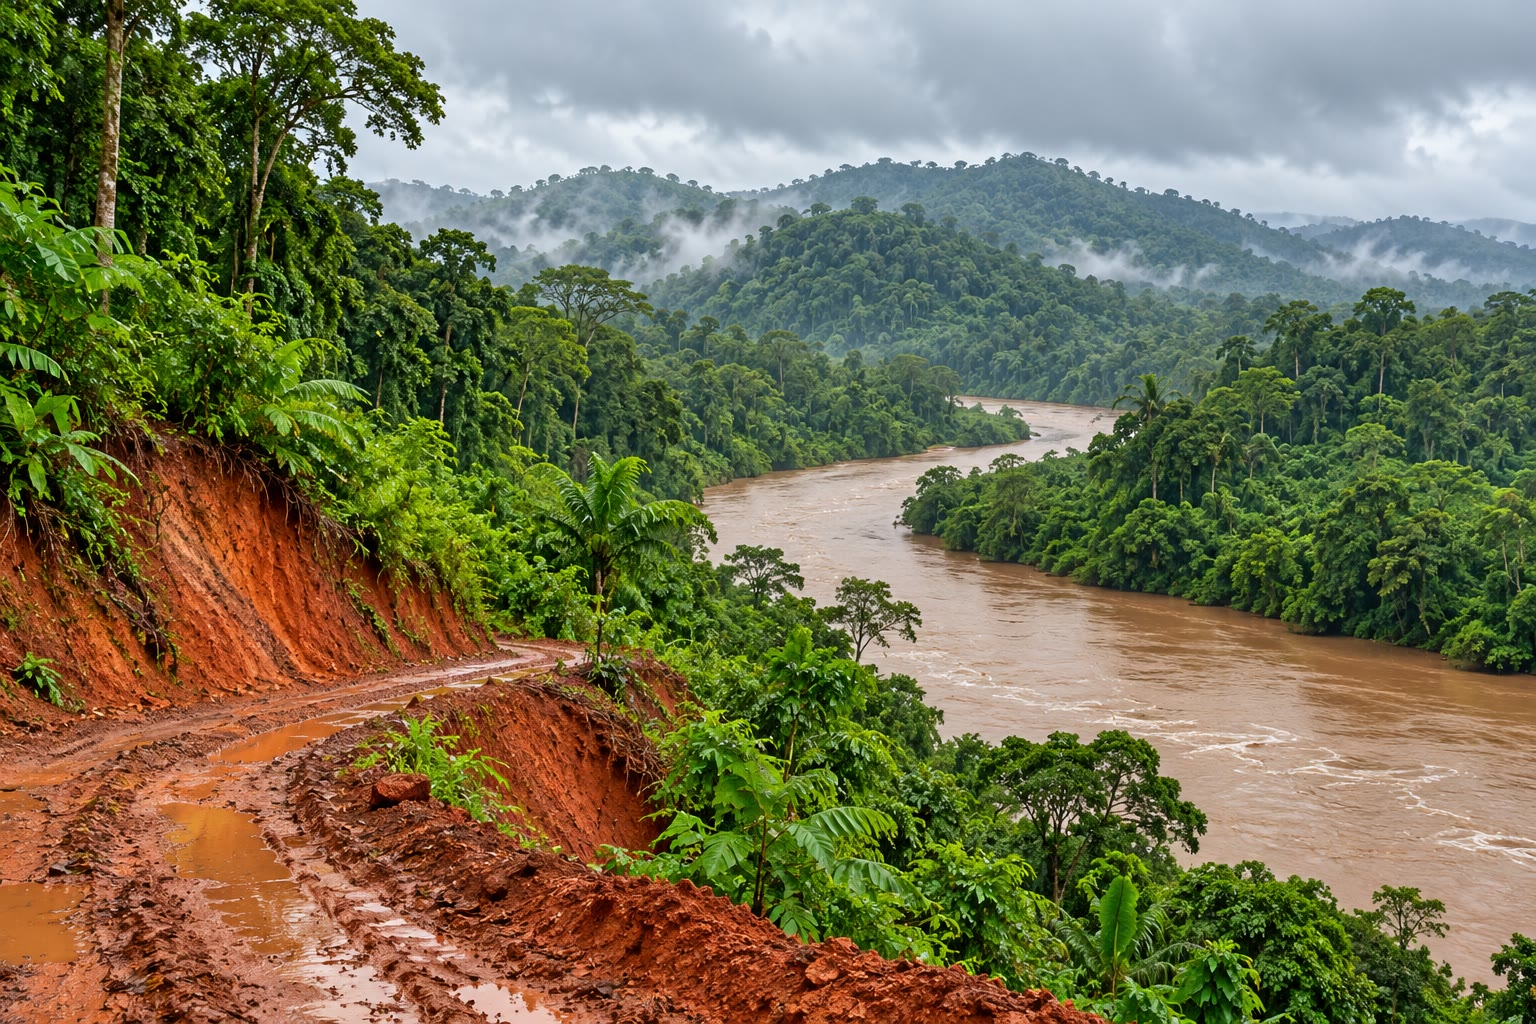
\includegraphics[width=0.66\linewidth]{images/book4/ai/b2-tropical-weathering.jpg}
\par\smallskip{\small حيث يعمل منظّم الحرارة بأقصى جهده: أرض منخفضة حارّة رطبة، يسقط فيها المطر على
تربة حمراء متجوّية بعمق ويحمل فيها النهر نواتج التجوية إلى البحر
(رسم توضيحي مولَّد بالذكاء الاصطناعي).}
\end{omfigure}

\section*{التمارين}\label{sec:b2:deep-time-climate:exercises}

معطيات التمارين، ما لم يُذكر غير ذلك: الكربون في الغلاف الجوي قبل الصناعة
\qty{591}{PgC} (\qty{278}{ppm})؛ و$\qty{1}{Tmol}$ من الكربون $= \qty{0.012011}{PgC}$؛ وتجوية
السيليكات $W_0 = \qty{0.138}{PgC.yr^{-1}}$؛ والحصّة الباقية في الهواء من فائض بعد عمل المحيط
والكربونات $f = 0.08$؛ وحساسية التجوية $k_T = \qty{0.09}{K^{-1}}$؛ وحساسية المناخ $S =
\qty{3}{K}$؛ وتأثير مضاعفة ثنائي أكسيد الكربون \qty{3.93}{W.m^{-2}}؛ و$R =
\qty{8.314}{J.mol^{-1}.K^{-1}}$.
% ledger: ar6ch5:fig512, ipcc:erf-2xco2, derry24:fluxes, colbourn13:timescale, colbourn13:weathering, ipcc:ecs

\begin{exercise}[$\star$]\label{exo:b2:deep-time-climate:1}
قبل العصر الصناعي كان المحيط يحتوي على \qty{900}{PgC} في طبقته السطحية، و\num{37100} في
مياهه المتوسطة والعميقة، و700 على هيئة كربون عضوي مذاب و3 في كائناته الحيّة.
(أ) كم كان المحيط يحتوي من الكربون، وكم مرّة قدر ما في الغلاف الجوي؟ (ب) حوّل
الكمّية \qty{3.5e6}{Tmol} في الخزّانات السطحية إلى بيتاغرامات من الكربون. (ج) ما الحصّة منها الموجودة في
الهواء؟
\end{exercise}

\begin{exercise}[$\star$]\label{exo:b2:deep-time-climate:2}
استعمل تدفّقات شكل \omterm{def:b2:deep-time-climate:carbon-cycle}{الدورة الطويلة الأمد للكربون}، مع أخذ انطلاق الغازات التحوّلي مساويًا
\qty{3}{Tmol.yr^{-1}}. (أ) اجمع المدخلات إلى الخزّانات السطحية والمخرجات.
(ب) ما حصّة المدخلات التي تقدّمها البراكين والوديان الخسفية والتحوّل؟ (ج) أوجد زمن
مكوث الكربون في الخزّانات السطحية، باستعمال المخرجات.
\end{exercise}

\begin{exercise}[$\star$]\label{exo:b2:deep-time-climate:3}
(أ) اكتب تجوية الفورستريت، \ce{Mg2SiO4}، بثنائي أكسيد الكربون والماء إلى أيونات المغنيسيوم
والبيكربونات والسيليكا المذابة، \ce{SiO2}، ووازنها. (ب) يترسّب المغنيسيوم لاحقًا
على هيئة كربونات. اكتب التفاعل الصافي. (ج) ما كتلة الفورستريت التي يجب أن تتعرّض للتجوية
لنزع \qty{1}{PgC} نهائيًا؟ ($M(\ce{Mg2SiO4}) = \qty{140.7}{g.mol^{-1}}$.)
\end{exercise}

\begin{exercise}[$\star$]\label{exo:b2:deep-time-climate:4}
رتّب بحسب العمر، مع تواريخها، وقل لكلّ منها هل كانت الأرض في حالة دفيئة أم في
حالة جليدية: الأمثل المناخي للإيوسين المبكّر؛ والتجلّد الهيرنانتي؛ وبداية
الغطاء الجليدي القطبي الجنوبي؛ والتوروني؛ وأقصى امتداد للجليد في أواخر الباليوزوي؛ والتقدّمات
الكبرى للأغطية الجليدية الشمالية؛ \omterm{def:b2:deep-time-climate:petm}{والحدّ الأقصى الحراري للباليوسين--الإيوسين}.
\end{exercise}

\begin{exercise}[$\star\star$]\label{exo:b2:deep-time-climate:5}
(أ) تحقّق من أن طاقة تنشيط قدرها \qty{63}{kJ.mol^{-1}} عند \qty{288}{K} تعطي $k_T =
\qty{0.09}{K^{-1}}$. (ب) أوجد $k_T$ للقيمة الميدانية \qty{74}{kJ.mol^{-1}}. (ج) أوجد مع كلّ منهما
الاحترار المستقرّ حين يرتفع انطلاق الغازات بنسبة \qty{20}{\percent}. (د) لماذا لا تدخل حساسية
المناخ في (ج)؟
\end{exercise}

\begin{exercise}[$\star\star$]\label{exo:b2:deep-time-climate:6}
قارن عامل أرينيوس الدقيق $\exp[-(E_{\text a}/R)(1/T - 1/T_0)]$ بالعامل $e^{k_T(T -
T_0)}$، $k_T = E_{\text a}/(RT_0^2)$، مع $E_{\text a} = \qty{63}{kJ.mol^{-1}}$ و$T_0 =
\qty{288}{K}$: (أ) عند $T = \qty{293}{K}$؛ (ب) عند $T = \qty{318}{K}$. (ج) بيّن أن نسبة
التقريب إلى العامل الدقيق هي $\exp[E_{\text a}x^2/(RT_0^2(T_0 + x))]$، مع $x = T - T_0$،
وأوجد الاحترار الذي تبلغ عنده 1.1.
\end{exercise}

\begin{exercise}[$\star\star$]\label{exo:b2:deep-time-climate:7}
تعطي التجميعة المنعّمة \qty{1444}{ppm} من ثنائي أكسيد الكربون عند \qty{419.5}{Ma}
و\qty{276}{ppm} عند نهاية سجلّها. (أ) أوجد تأثير هذا الانخفاض. (ب) قارنه
بالقيمة \qty{9}{W.m^{-2}} للشمس المتزايدة سطوعًا. (ج) أوجد المعدّل المتوسط للانخفاض بوحدة ppm لكلّ مليون
سنة، وقارنه بالقيمة \qty{3.4}{ppm} للاتجاه الملائم. لماذا قد يختلفان؟
\end{exercise}
% ledger: data:b4-foster2017, foster17:co2

\begin{exercise}[$\star\star$]\label{exo:b2:deep-time-climate:8}
(أ) وزّع \num{3000} و\qty{7000}{PgC} على 3 وعلى \qty{20}{kyr}: ما مدى معدّلات
الإطلاق الناتج؟ قارن بالمدى 0.3 إلى \qty{1.5}{PgC.yr^{-1}} الذي تذكره الهيئة الحكومية الدولية. (ب) كانت الانبعاثات البشرية
نحو \qty{35}{Gt} من ثنائي أكسيد الكربون عام 2010. حوّلها إلى كربون وقارن. (ج) ارتفع ثنائي أكسيد
الكربون من 900 إلى \qty{2000}{ppm}. أوجد التأثير والاحترار عند التوازن مع $S =
\qty{3}{K}$، وقارن بالاحترار البالغ \qty{5}{\celsius} فوق المناخ السابق للحدث.
\end{exercise}
% ledger: ar6ch5:petm-release, usgs:volcanic-co2, ar6ch5:petm

\begin{exercise}[$\star\star$]\label{exo:b2:deep-time-climate:9}
يضاعف نهوض حزام جبلي قابليةَ الأرض للتجوية $W_0$ بالعامل 1.2، مع انطلاق غازات
ثابت. (أ) أوجد التغيّر الجديد في درجة الحرارة المستقرّة. (ب) أوجد ثنائي أكسيد الكربون المستقرّ الجديد، انطلاقًا من
\qty{278}{ppm}. (ج) هل يختلف معدّل تجوية السيليكات، في الحالة المستقرّة الجديدة، عن
المعدّل القديم؟ علّل.
\end{exercise}

\begin{exercise}[$\star\star\star$]\label{exo:b2:deep-time-climate:10}
(أ) أوجد زمن الاضمحلال الأسّي لمنظّم الحرارة مع عامل الجريان السطحي، $k = 0.09 + 0.65\times0.045$.
(ب) على مدى ملايين السنين تستجيب الأغطية الجليدية والنباتات أيضًا؛ فمع حساسية لنظام الأرض
قدرها \qty{8}{K} لكلّ مضاعفة بدلًا من $S$، أوجد $\tau$ مع $k_T$. (ج) في أيّ اتجاه يدفع
التغييران منظّم الحرارة، وأيّ الشكّين أهمّ، $E_{\text a}$ أم $S$؟
\end{exercise}

\begin{exercise}[$\star\star\star$]\label{exo:b2:deep-time-climate:11}
إطلاق \qty{5000}{PgC} (بعد عمل المحيط والكربونات). (أ) أوجد ثنائي أكسيد الكربون في
الهواء، بوحدة ppm، والاحترار. (ب) أوجد معدّل النزع الصافي الابتدائي $W - W_0$، والزمن الذي
تستغرقه النبضة لتختفي بهذا المعدّل. (ج) أوجد الزمن الخطّي اللازم لنزع \qty{90}{\percent}
من الفائض. (د) يستغرق النموذج، إذا كومل دون جعله خطّيًا، \qty{340}{kyr}. لماذا أطول؟
\end{exercise}

\begin{exercise}[$\star\star\star$]\label{exo:b2:deep-time-climate:12}
(أ) اجعل النموذج خطّيًا حول حالة مستقرّة يكون فيها انطلاق الغازات $V$ و$C = C^*$، وبيّن أن
زمن الاضمحلال الأسّي هو $\tau' = A_0 (C^*/C_0)\ln 2/(f k S V)$. (ب) احسبه للحالة المستقرّة
الناتجة عن ارتفاع انطلاق الغازات بنسبة \qty{20}{\percent}. (ج) هل منظّم الحرارة أسرع أم أبطأ في عالم غنيّ
بثنائي أكسيد الكربون، ولماذا؟
\end{exercise}

\begin{problem}[{مسألة نهاية الأسبوع --- كم يستغرق منظّم الحرارة؟}]\label{pb:b2:deep-time-climate:1}
تبني هذه المسألة الثابت الزمني لمنظّم الحرارة من تدفّقات مقيسة. استعمل معطيات
التمارين؛ وانطلاق الغازات عند الظهرات والجزر المحيطية والأقواس والوديان الخسفية \num{1.3} و\num{1.3} و4.5
و\qty{4.2}{Tmol.yr^{-1}}؛ وتجوية السيليكات من 11 إلى \qty{12}{Tmol.yr^{-1}}؛ وطاقة التنشيط
\qty{63}{kJ.mol^{-1}} عند $T_0 = \qty{288}{K}$؛ وكتلة الغلاف الجوي \qty{5.1e18}{kg}، والكتلة المولية
المتوسطة للهواء \qty{28.97}{g.mol^{-1}}. قرّب إلى ثلاثة أرقام معنوية.

\noindent\textbf{الجزء الأول --- الموازنة.}
\begin{enumerate}
  \item اجمع انطلاق الغازات من البراكين والوديان الخسفية، بوحدة \unit{Tmol.yr^{-1}} وبوحدة \unit{PgC.yr^{-1}}.
  \item خذ $W_0$ في منتصف مداه؛ وحوّله إلى \unit{PgC.yr^{-1}}.
  \item قارن بينهما. ماذا توحي المقارنة بشأن \omterm{def:b2:deep-time-climate:carbon-cycle}{الدورة الطويلة الأمد للكربون}؟
  \item كم مولًا من الهواء يحتوي الغلاف الجوي؟ وكم مولًا من الكربون في \qty{591}{PgC}،
        وما نسبة الخلط الموافقة؟
  \item من دون أيّ تجوية على الإطلاق، كم يستغرق انطلاق الغازات في السؤال 1 ليضيف
        \qty{591}{PgC} إلى الخزّانات السطحية؟
  \item إذا بقي الكسر $f = 0.08$ من ذلك في الهواء، فبأيّ عامل يرتفع ثنائي أكسيد الكربون
        في الهواء؟
\end{enumerate}

\noindent\textbf{الجزء الثاني --- الجعل الخطّي.}
\begin{enumerate}[resume]
  \item أوجد $k_T$ من طاقة التنشيط، وتحقّق من أنها تُقرَّب إلى القيمة
        \qty{0.09}{K^{-1}} المستعملة أدناه.
  \item بأيّ عامل تزداد التجوية لاحترار قدره \qty{1}{K}؟
  \item اكتب الاحترار $\Delta T$ لفائض $M$، ومشتقّه عند $M = 0$، بوحدة
        \unit{K.PgC^{-1}}.
  \item أوجد مشتقّ $W$ بالنسبة إلى $M$ عند $M = 0$، بوحدة \unit{yr^{-1}}.
  \item بيّن أن مقلوبه هو الثابت الزمني $\tau$ في
        \cref{prop:b2:deep-time-climate:thermostat}.
  \item أيّ الكمّيات $f$ و$k$ و$S$ و$W_0$ تجعل منظّم الحرارة أسرع حين تزداد؟
\end{enumerate}

\noindent\textbf{الجزء الثالث --- الثابت الزمني.}
\begin{enumerate}[resume]
  \item احسب $\tau$.
  \item احسبه مع عامل الجريان السطحي، $k = \qty{0.119}{K^{-1}}$.
  \item احسبه مع $k_T$ وطاقة تنشيط قدرها \qty{74}{kJ.mol^{-1}}.
  \item قارن هذه القيم بالمدى من \qty{200}{kyr} إلى \qty{1}{Myr} في النماذج التي تمثّل المحيط صراحةً.
  \item كم زمنَ اضمحلال أسّيًا يتّسع له مدى \qty{50}{Myr} لانخفاض ثنائي أكسيد الكربون في
        السينوزوي؟ وماذا يقول ذلك عن حالة دورة الكربون خلال الانخفاض؟
  \item بمعدّل \qty{16}{ppm} لكلّ مليون سنة، كم يتغيّر ثنائي أكسيد الكربون في مدّة $\tau$ واحدة؟
\end{enumerate}

\noindent\textbf{الجزء الرابع --- إطلاق بحجم الحدّ الأقصى الحراري.}
\begin{enumerate}[resume]
  \item أُطلق \qty{5000}{PgC}؛ كم يبقى منه في الهواء بعد أن يعمل المحيط والكربونات،
        وما ثنائي أكسيد الكربون بوحدة ppm؟
  \item أوجد الاحترار في تلك اللحظة.
  \item بكم يرتفع معدّل التجوية، بوحدة \unit{PgC.yr^{-1}} وبالنسبة المئوية؟
  \item بالقانون الخطّي، كم يمضي من الزمن حتى يزول \qty{90}{\percent} من الفائض؟
  \item تعافت كربونات الحدّ الأقصى الحراري على مدى نحو \qty{100}{kyr}. اذكر سببين يجعلان الأرض
        الحقيقية ربّما أسرع من هذا النموذج.
  \item خلاصة القول: ما زمن الاضمحلال الأسّي \omterm{def:b2:deep-time-climate:thermostat}{لمنظّم الحرارة بتجوية السيليكات} في هذا النموذج؟
\end{enumerate}
\end{problem}
% ledger: derry24:fluxes, colbourn13:weathering, colbourn13:timescale, ar6ch5:fig512, ar6ch5:petm, ar6ch5:cenozoic-co2, ipcc:ecs, earth:Matm, earth:Mmol
